% -----------------------------------------------
% Template for ISMIR Papers
% 2020 version, based on previous ISMIR templates

% Requirements :
% * 6+n page length maximum
% * 4MB maximum file size
% * Copyright note must appear in the bottom left corner of first page
% * Clearer statement about citing own work in anonymized submission
% (see conference website for additional details)
% -----------------------------------------------

\documentclass{article}
\usepackage[T1]{fontenc} % add special characters (e.g., umlaute)
\usepackage[utf8]{inputenc} % set utf-8 as default input encoding
\usepackage{ismir,amsmath,cite,url}
\usepackage{graphicx}
\usepackage{color}
\usepackage[bookmarks=false]{hyperref}
\usepackage{multirow}
\usepackage{xcolor}
\usepackage{soul}

% Optional: To use hyperref, uncomment the following.
% \usepackage[bookmarks=false,hidelinks]{hyperref}
% Mind the bookmarks=false option; bookmarks are incompatible with ismir.sty.

\usepackage{lineno}
% \linenumbers

\makeatletter
\newcommand{\printfnsymbol}[1]{%
%   \textsuperscript{\@fnsymbol{#1}}%
  \textsuperscript{*}%%
}
\makeatother

\newcommand\blfootnote[1]{%
  \begingroup
  \renewcommand\thefootnote{}\footnote{#1}%
  \addtocounter{footnote}{-1}%
  \endgroup
}

% Title.
% ------
\title{``Butter Lyrics Over Hominy Grit''\textsuperscript{\textdagger}: Comparing Audio and Psychology-Based Text Features in MIR Tasks}

% Note: Please do NOT use \thanks or a \footnote in any of the author markup

% Single address
% To use with only one author or several with the same address
% ---------------
%\oneauthor
% {Names should be omitted for double-blind reviewing}
% {Affiliations should be omitted for double-blind reviewing}

% Two addresses
% --------------
%\twoauthors
%  {First author} {School \\ Department}
%  {Second author} {Company \\ Address}

%% To make customize author list in Creative Common license, uncomment and customize the next line
%  \def\authorname{First Author, Second Author}


% Three addresses
% --------------
%\threeauthors
%  {First Author} {Affiliation1 \\ {\tt author1@ismir.edu}}
%  {Second Author} {\bf Retain these fake authors in\\\bf submission to preserve the formatting}
%  {Third Author} {Affiliation3 \\ {\tt author3@ismir.edu}}

%% To make customize author list in Creative Common license, uncomment and customize the next line
%  \def\authorname{Jaehun Kim, Andrew M. Demetriou, Sandy Manolios, Cynthia C.S. Liem, Stella M. Tavella}

% Four or more addresses
% OR alternative format for large number of co-authors
% ------------
\multauthor
{Jaehun Kim$^1$\thanks{Authors contributed equally to the work.} \hspace{1cm} Andrew M. Demetriou$^1$\printfnsymbol{1} \hspace{1cm} Sandy Manolios$^1$} { \bfseries{ M. Stella Tavella$^2$ \hspace{1cm} Cynthia C.~S. Liem$^1$ \hspace{1cm}}\\
  $^1$ Delft University of Technology, Netherlands\\
$^2$ Musixmatch, Bologna, Italy\\
{\tt\small J.H.Kim@tudelft.nl}\\
{\tt\small A.M.Demetriou@tudelft.nl}
}
  \def\authorname{Jaehun Kim, Andrew M. Demetriou, Sandy Manolios, Stella M. Tavella, Cynthia C.~S. Liem}


\sloppy % please retain sloppy command for improved formatting

\begin{document}

%
\maketitle
%
\begin{abstract}
Psychology research has shown that song lyrics are a rich source of data, yet they are often overlooked in the field of MIR compared to audio. In this paper, we provide an initial assessment of the usefulness of features drawn from lyrics for various fields, such as MIR and Music Psychology. To do so, we assess the performance of lyric-based text features on 3 MIR tasks, in comparison to audio features. Specifically, we draw sets of text features from the field of Natural Language Processing and Psychology. Further, we estimate their effect on performance while statistically controlling for the effect of audio features, by using a hierarchical regression statistical model. Lyric-based features show a small but statistically significant effect, that anticipates further research. Implications and directions for future studies are discussed. 
\end{abstract}
%
\section{Introduction}
\label{sec:introduction}
% intro / motivation / what we do / etc.
\blfootnote{\textsuperscript{\textdagger}Quoted words are lyrics written by Clifford Smith, from the song ``The What'', by the Notorious B.I.G. featuring Methodman, on the album ``Ready to Die'', released in 1994.}Popular Western music very often contains lyrics. Social science research has shown informative relationships between popular songs and their lyrical content: e.g., country music lyrics rarely include political concepts \cite{van2005world}, songs with more typical \cite{north2020relationship} and more negative \cite{brand2019cultural} lyrics appear to be more successful, and the psychological content of song lyrics appears to correlate with cultural changes in psychological traits \cite{dewall2011tuning}. As for music consumption, lyrics have also been shown to be a salient component of music in the minds of listeners \cite{demetriou2018vocals}. Furthermore, \cite{howlin2020patients} showed that patients are more likely to choose music with lyrics when participating in music-based pain reduction interventions; \cite{ali2006songs} showed that lyrics enhance self reported emotional responses to music, although melody had an overall larger effect, and \cite{brattico2011functional} showed a number of additional brain regions were active during the listening of sad music with lyrics, vs.\ sad music without lyrics. 

In the Music Information Retrieval (MIR) field, some interest for lyrics and how they can be used to improve MIR tasks has been shown. Popular uses of lyrics for MIR tasks consider mood classification \cite{hu2010lyrics,mcvicar2011mining, hu2009lyric,wang2011music}, genre classification \cite{mayer2008rhyme,tsaptsinos2017lyrics} and topic detection for indexing and browsing \cite{kleedorfer2008oh, sasaki2014lyricsradar}. \cite{ellis2015quantifying} also proposed a metric to assess the novelty of lyrics, and suggested that novelty can play a role in music preference.

From these findings, one can conclude that lyrics are a rich data source. Although MIR interests have historically focused more on audio, lyrics information may fruitfully be leveraged for various MIR tasks. Still, there are many possible ways to extract information from lyrics text, and it is an open question what information extraction procedure will turn out most fruitful. To gain more insight into this, we present a study investigating several textual feature sets. In shaping these sets---acknowledging potential value of the topic for social science research---we are inspired by the way text analysis has been performed in the Psychology domain, and draw several of our extractors from prior work in that field. We will assess the performance of these textual feature sets on 3 common MIR tasks, and will statistically control for the effect of each chosen feature set, including an audio feature set for comparison.
Our analysis will be performed on a large dataset from the online Musixmatch lyrics catalogue.

In the remainder of the paper, in Section~\ref{sec:relatedworks}, we discuss relevant previous work on text information extraction in the Psychology literature. Section~\ref{sec:resdes} will subsequently explain our research design, after which Section~\ref{sec:featset} discusses the feature sets we used. Section~\ref{sec:data} describes the data collection and pre-processing procedures, after which Section~\ref{sec:exp} details the experimental design. Section~\ref{sec:analysis} justifies our chosen analytical strategy, followed by a presentation of results in Section~\ref{sec:result} and the conclusion in Section~\ref{sec:conclusion}.

%Prior research therefore suggests lyrics are a rich data source that, perhaps along with insights from Psychology, may be fruitfully leveraged for various tasks in the field of MIR. We explore this claim by: \hl{1) drawing the text based features from prior work in Psychology as well as more contemporary NLP work, 2) statistically controlling for the effect of audio features in our analysis, 3) assessing the performance of text-based features on 3 common MIR tasks},  4) using a large dataset collected by musixmatch, an online lyrics catalog. Following in section 2 is a discussion of prior work, and the psychological feature sets we employed in our study. Section 3 discusses how musixmatch collects data, and how the dataset for our analysis was drawn. Section 4 describes our experimental setup, section 5 describes our statistical approach. Results and conclusions are discussed in sections 6 and 7 respectively. 

\section{Related Work}\label{sec:relatedworks}
% literature review for the constructs and some MIR papers using lyrics
The field of Psychology has long pondered the importance of the words people choose to use, and how this reflects their individual differences \cite{tausczik2010psychological}.
%In this section, we discuss the psychology-based features we extract from lyrics. 
The features we use in present work are primarily inspired by two prior lines of work in which Natural Language Processing (NLP) techniques were applied in psychology research: one employing closed-vocabulary lexicon approaches, the other employing open vocabulary approaches. Firstly, \cite{neuman2016personality} used NLP techniques to derive estimates of personality for music genres. Specifically, they created a lexicon (a meaningful group of words) from psychology research that described personality dimensions, as well as a corpus of lyrics, separated into music genres.  They then computed the similarity between the lyrics of music genres and the groups of personality dimension words, and considered this result to be an estimate of the personality dimension represented in the lyrics of each genre. Lexicon-based approaches have generally been popular, also thanks to the release of the Linguistic Inquiry Word Count (LIWC) lexicon-based software~\cite{pennebaker2015development}; e.g., in the context of lyrics,~\cite{markowitz201727} used it to examine psychological distress in the lyrics of musicians that committed suicide vs.\ those who had not. 
%Following this approach, we curate groups of words related to psychological characteristics, and extract similarity scores between these word groups and lyrics. 

Secondly, \cite{schwartz2013personality} demonstrated the usefulness of an open vocabulary approach vs.\ a lexicon approach while examining personality in the context of online social networks. Although lexicons are carefully curated and meaningful, they are also time-consuming to create and context-specific. In contrast, data-driven techniques can automatically estimate latent topics from groups of words that tend do appear together. \cite{schwartz2013personality} showed relationships between personality scores and automatically extracted latent topics. Further, they showed that the open vocabulary approach may have stronger correlations to self-reported personality scores than the closed-vocabulary lexicon approaches. 

% \subsection{Psychology-Based Features}
%  \subsubsection{LIWC}
% Linguistic Inquiry Word Count (LIWC) is a software package built on a lexicon that has been validated for text analysis in psychological studies \cite{pennebaker2014development}, including lyrics: e.g. \cite{markowitz201727} who used it to examine psychological distress in the lyrics of musicians that committed suicide vs. those who had not. Specifically, the LIWC is a curated lexicon, separated into 73 categories e.g. Social Processes, such as references to family and friends, Psychological processes, such as reference to emotions, Drives, such as risk and reward etc. The software outputs the counts of words in a given text per each of the 73 categories. 

% \subsubsection{Personality}
%  Contemporary personality theory is derived from lexical studies: it has been suggested that meaningful individual psychological differences between people are captured in the adjectives that describe people \cite{goldberg1990alternative}. Although the number of meaningful clusters of adjectives (called Personality Dimensions) is under debate, the OCEAN or Big-Five model is often used. It is composed by 5 traits : Openness to Experience, Conscientiousness, Extroversion, Agreeableness and Neuroticism \cite{goldberg1990alternative}. Our Personality feature set consisted of 2 word groups per dimension, comprised of words representing positive and negative aspects of each personality dimension, derived from prior research \cite{saucier1996evidence}.

% \subsubsection{Personal Values}
% Personal values are another important component of identity, though less studied. They are stable over time and represents who people want to be, what are the most important things for them in life at the most abstract level. The traditional way to obtain people's personal values is through questionnaires but recent works focused on NLP techniques to extract them from text \cite{wilson2016disentangling,wilson2018building,liu2019personality}. In our work, we used the value inventory and lexicon from \cite{wilson2018building}. 

\section{Research Design}\label{sec:resdes}

\begin{figure}[!tb]
    \centering
    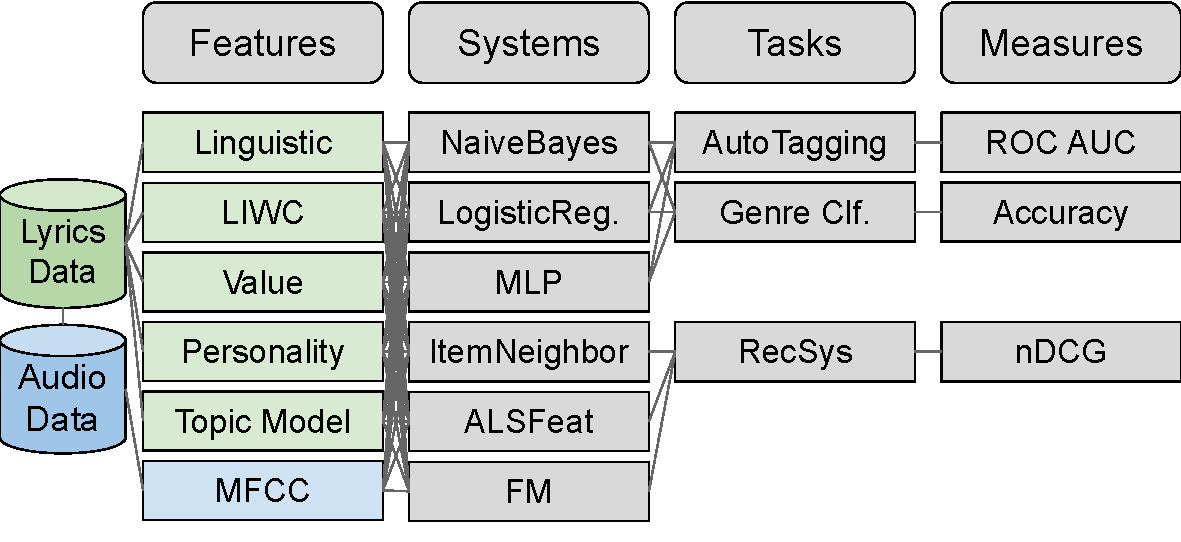
\includegraphics[width=0.9\linewidth]{latex/figs/LyricPsych_Overview.pdf}
    \caption{Overview of the experimental pipeline.}
    \label{fig:experimental_pipeline}
\end{figure}

% overview
In this study, we seek to examine the relative importance of lyric-based text features---especially features drawn from psychology research--- for various popular MIR tasks. We wish to compare this importance to that of conventional audio based features.

An overview of our experimental pipeline is given in Figure~\ref{fig:experimental_pipeline}. Various feature sets will feed into various systems, that are appropriate for various MIR machine learning tasks. We employ a full-factorial experimental design for feature sets, tasks, and the systems attached to each task, which means we research all the possible combinations of those factors. For each combination, we will employ the traditional train-validation-test machine learning setup. Performance results on the test sets will feed into our statistical analysis, where we will explicitly control for the effect of each of the feature sets.

%from the combinatorial pool, a task simulation is conducted, where the features corresponding to the data points within the training set dataset are used to develop a system automatically, where the hyper-parameter tuning with the validation set may be applied, tested by the held-out dataset with respect to the accuracy measurement for each task. The simulation setup for each case and the performance measure is recorded as the further statistical analysis, where the desired experimental result we seek is investigated in systematic way.

%We first consider a number of psychologically oriented features based on the prior research as discussed in Section~\ref{sec:relatedworks}. To examine the relative effectiveness of each feature considered to MIR tasks, we setup and execute a set of task simulation runs. Specifically, we select 3 popular MIR tasks including the auto-tagging, genre classification and music recommendation and systems that are commonly used for each task. Although the development process of each task is not perfectly aligned, we homogenize it by employing the conventional machine learning based system development practice. It implies that the system is developed on a set of dataset and validated by the held-out data points, and tested on the unseen future data, which is often simulated as the data split strategy such as the cross validation. The overview of the research design is illustrated in Figure~\ref{fig:experimental_pipeline}.



%\textcolor{red}{Jay:ANALYTICS STRATEGY HERE?}





\section{Feature Sets}\label{sec:featset}

% 1. Feature sets
In this work, we will consider 5 lyric-based text feature sets and an audio-based feature set. More details are given in the following subsections; a summary of the dimensionalities of all feature sets is given in Table~\ref{tab:feat_dim}.

\subsection{Linguistic Features}\label{sec:featset:lingfeat}
%   1.1. Linguistic Features
As baseline textual features for this study, we first extract several simple \emph{linguistic} features:

\begin{itemize}
    \itemsep0em 
    \item \emph{NumWords:} the number of words included in the lyrics text.
    \item \emph{NumUniqueWords:} the number of  unique words in the lyrics text.
    \item \emph{NumStopWords:} the number of stop words in the lyrics text\footnote{As we will focus on English lyrics in this study, we used the English stop words corpus from the Natural Language Toolkit (NLTK)~\cite{DBLP:books/daglib/0022921}}.
    \item \emph{NumRareWords} the number of words that appeared in less than $5$ lyrics.
    \item \emph{NumCommonWords} the number of  words extremely commonly used within a lyrics corpus. We set the threshold as the 30\% percentile of the document frequency of words.
\end{itemize}

Along with the absolute number, we also compute the ratio over the total number of words for each lyrics text. 

\subsection{Topic Modeling}\label{sec:featset:topic}
%   1.2. Topic Model (Open Vocabulary)

As a more advanced feature extraction technique, we employ probabilistic Latent Semantic Analysis (pLSA)~\cite{DBLP:journals/ml/Hofmann01} for \emph{topic} modeling. We treat each of the lyric texts as a document, and will take the found topic distribution for a given document as the document feature. We chose the number of topics $K=25$, which maximizes validation log-perplexity. Taking advantage of the unsupervised learning setup, we use the total pool of songs to setup the training-validation-test split.

\subsection{LIWC}\label{sec:featset:LIWC}
%   1.3. LIWC (Closed Vocabulary)
Linguistic Inquiry Word Count (LIWC) is a software package built on a lexicon that has been validated for text analysis in psychological studies \cite{pennebaker2015development}. It uses a curated lexicon, separated into 73 categories (e.g., the category `Social Processes' includes references to family and friends). The software outputs the counts of words in a given text for each of the 73 categories. We employ the latest LIWC, released in 2015. 
% Details on the indexing methods (trie)

\subsection{Psychology Inventory Scores}\label{sec:featset:inventory_scores}

We will consider two more feature sets, inspired by psychology inventory scores: a feature set focusing on \emph{personality} and a feature set focusing on \emph{values}. In both cases, we will use lexicons from literature. However, rather than performing a word count as was done in LIWC, we will use more contemporary NLP techniques based on word embeddings.

Contemporary personality theory is derived from lexical studies: it has been suggested that meaningful individual psychological differences between people are captured in the adjectives that describe people \cite{goldberg1990alternative}. Although the number of meaningful clusters of adjectives (called Personality Dimensions) is under debate, the OCEAN or Big-Five model is often used. It is composed of 5 traits : Openness to Experience, Conscientiousness, Extroversion, Agreeableness and Neuroticism~\cite{goldberg1990alternative}. Our \emph{personality} feature set consists of 2 word clusters per dimension, comprised of words representing positive and negative aspects for each personality dimension, derived from prior research \cite{saucier1996evidence}.

Personal \emph{values} are another important component of identity, though less studied. They are stable over time and represent who people want to be, targeting the most important things for them in life at the most abstract level. The traditional way to obtain people's personal values is through questionnaires, but recent works focused on NLP techniques to extract them from text~\cite{wilson2016disentangling,wilson2018building,liu2019personality}. In our work, we used the value inventory and lexicon from~\cite{wilson2018building}. 

Both for the \emph{personality} and \emph{values} feature sets, we will exploit the \texttt{word2vec} model~\cite{DBLP:conf/nips/MikolovSCCD13} to approximate distances between lyrics and the various inventory categories in the feature sets. For this, we use the model pre-trained on the Google News dataset\footnote{\url{https://code.google.com/archive/p/word2vec/}}. 
The average distance score $s_{d,c}$ for each lyric text $d$, and category $c$ is computed by taking the average cosine distance between the words belonging to the lyrics and the categories, respectively:
\begin{equation}
    s_{d, c} = \frac{1}{|\mathcal{W}_d||\mathcal{W}_c|}\sum_{n\in\mathcal{W}_d}\sum_{m\in\mathcal{W}_c} \frac{\langle \mathbf{v}_n, \mathbf{v}_m \rangle}{||\mathbf{v}_n|| \cdot ||\mathbf{v}_m||}
\end{equation}
where $\mathcal{W}_d$ and $\mathcal{W}_c$ represent the set of words belonging to the lyrics text $d$ and the category $c$. $v_n$ and $v_m$ denote the pre-trained word vectors corresponding to word $n$ in the lyrics and word $m$ in the category, respectively.


\subsection{MFCC}\label{sec:featset:mfcc}
%   1.6. Audio Features

Finally, we employ a set of audio features based on the Mel-Frequency Cepstral Coefficients (MFCC). We include these, such that the effect of the lyric-based text features can be compared to a commonly used feature set from the primary modality of interest in many MIR tasks. Specifically, we adopt the feature computation introduced in~\cite{DBLP:conf/ismir/ChoiFSC17} with $40$ mel bins. 

\begin{table}[!tb]
\centering
\begin{tabular}{ccc}
% \hline
Feature Set & Dimensions\\ \hline
Audio & \ 240   \\
LIWC & \ 73 \\
Values  & \ 49   \\ 
Topics  & \ 25   \\
Personality  & \ 10   \\ 
Linguistic  & \ 9   \\ 
\end{tabular}
\caption{Number of dimensions per feature set}
\label{tab:feat_dim}
\end{table}

\section{Data Collection}\label{sec:data}
%  / details

We analyzed the lyrics contained in the Musixmatch dataset\footnote{\url{http://millionsongdataset.com/musixmatch/}}, which is the official lyrics metadata selection integrated in the Million Song Dataset (MSD) ~\cite{DBLP:conf/ismir/Bertin-MahieuxEWL11}, a collection of relevant data and metadata for one million popular contemporary songs.
\href{https://www.musixmatch.com/}{Musixmatch} is a lyrics and music language platform. The Musixmatch community drives the content production by adding, correcting, syncing and translating lyrics of songs. The process of lyrics quality verification involves several steps, including spam detection, formatting, spelling and translation checking. These steps are accomplished by the use of both artificial intelligence and machine learning models. In addition, they are manually verified by more than $2000$ Curators worldwide, and a local team of Musixmatch Editors, who are native speakers in different languages.

The data used for the purpose of this project consists of $182,808$ lyrics, plus relevant metadata such as the unique identifier, artist and title. The data encompasses $20,219$ unique artists over various genres of music.


\subsection{Preprocessing}\label{sec:setup:preproc}
% preprocessing (English entry filtering / stemming / tekenizing / ETC)
For the given lyrics dataset, we consider the following preprocessing steps: the sentence strings are 1) tokenized and 2) lemmatized, followed by 3) stop-words filtering and 4) filtering extremely rare and extremely common words (see Section~\ref{sec:featset:lingfeat}). Finally, we filter out non-English lyrics by a filtering process using the topic modeling. More precisely, we fit the topic model to detect whether the topics contain non-English words above a certain threshold. Songs that mostly load on non-English topics are removed.


\section{Experiment}\label{sec:exp}
% technical details on the pipelines (Jay)

\subsection{Tasks \& Systems}\label{sec:exp:task}
% 2. Tasks & Systems

As shown in Figure~\ref{fig:experimental_pipeline}, to assess the lyrics feature set, we consider $3$ popular MIR machine learning tasks; for each of these, we use $3$ different commonly used types of systems, and a task-specific performance measure is considered, as detailed below.

\subsubsection{Music Genre Classification}\label{sec:exp:task:genre}
%   2.1. Music Genre Classification
%     2.1.1. Systems: {LR, RF, MLP, Baselines[Random, MP]}
%     2.1.2. Measurement: Accuracy
%     2.1.3. Dataset: MxM genre
Music Genre Classification (MGC) is a multi-class classification problem. Typically, a set of music genres is given as the classes, and music audio content or features are used as the observations. In this study, we examine $3$ machine learning based systems: \emph{Gaussian Naive Bayes} (GNV), \emph{Logistic Regression} (LR) and the \emph{Multi-Layer Perceptron} (MLP).
% Along with the main systems of interests, we also test baselines such as the random classifier either following the class distribution of the uniform distribution.
For performance quantification, we opt for \emph{classification accuracy}.

For this task, we use the data in the intersection between our lyrics database and the part of the MSD for which the music genre mapping introduced in \cite{DBLP:conf/ismir/Schreiber15} can be made. By choosing the intersection with the MSD, our audio features can be extracted from the MSD preview audio excerpts. Due to genre label availability, this leads to $67,719$ songs being used in this task.

\subsubsection{Music Auto-Tagging}\label{sec:exp:task:autotagging}
%   2.2. Music Auto-Tagging 
%     2.2.1. Systems: {LR, RF, MLP, Baselines[Random, MP]}
%     2.2.2. Measurement: AUC^track
%     2.2.3. Dataset: MxM * MSD-Lastfm
Music Auto-Tagging (MAT) is often formulated as a multi-label classification problem in which multiple positive labels may exist for one input music observation. We used the same set of systems as in the MGC task\footnote{We employ a one-vs-rest strategy for the LR and GNV, which transforms a multi-label classification problem to multiple binary classification problems.}. Again, we cross-match to the MSD, now also considering MSD's LastFM social tags. Similarly to~\cite{DBLP:conf/ismir/ChoiFSC17}, we choose to focus on the $50$ most frequent tags from the dataset. The \emph{Area Under Curve - Receiver Operating Characteristic} (AUC-ROC) is used as the performance measure, which will be referred to as $AUC^{song}$ for the rest of this paper\footnote{We employed song-wise aggregation for this study}. Due to tagging label availability, $137,095$ songs are used under this task.

\subsubsection{Music Recommendation}\label{sec:exp:task:recsys}
%   2.3. Music Recommendation
%     2.3.1. Systems: {uNN, iNN, FM, Baselines[Random, MP, WRMF]}
%     2.3.2. Measurement: nDCG@100
%     2.3.3. Dataset: MxM * MSD-Echonest
Finally, Music Recommendation (MR) is considered for a user-related retrieval task. In particular, we consider a cold-start scenario, in which a batch of songs is newly introduced to the market, and required to be recommended to users. Due to the lack of previous interaction history, in such a scenario, a model will be maximally dependent on item attributes.
As this is a substantially different type of task than the previous classification tasks, a different set of the systems common to the recommender systems field is used. \emph{Item Nearest Neighbor} (INN) is a memory-based collaborative filtering method, which recommends the items closest to those that the user had consumed. We employ the feature vector introduced in Section~\ref{sec:featset} to compute the distance between entities using the cosine distance. We also use the \emph{Feature-augmented Matrix Factorization} (FMF)~\cite{DBLP:conf/ismir/LiangZE15} method, as well as the \emph{Factorization Machine}~\cite{DBLP:conf/icdm/Rendle10} (FM). These models are more sophisticated collaborative recommenders, which also are capable of exploiting item attributes.
% As for the baselines, we use the similar random baselines as the other tasks, which suggest songs randomly either from uniform or the song frequency. Additionally, we also present the \emph{Weighted Regularized Matrix Factorization} (WRMF) as the strong baseline where only the user-item interaction is employed.
The systems are developed and evaluated using the MSD-Echonest dataset~\cite{DBLP:conf/ismir/Bertin-MahieuxEWL11}. Due to limits on available computational resources, we exploit a densified subset with $96,551$ users and $66,850$ songs from the initial song pool with the lyrics\footnote{We initially matched the original Echonest dataset to our initial song pool and $30\%$ of randomly sampled users. Consequentially, we apply a filter, such that users who interacted with more than $5$ songs remain, and vice versa for songs.}. Finally, the binarized \emph{normalized Discounted Cumulative Gain} (nDCG) is considered as performance measure, for the top-$100$ songs recommended.

\subsection{Task Simulation Setup}\label{sec:exp:task:setup}
% description about the data-split / hyper-parameter search
All MIR tasks above are machine learning tasks, but the systems and data we choose to use for them did not yet exist in a real-life system. Therefore, we ran the machine learning procedures to initiate them. For this, for each task, we randomly split the available song data into \textit{training}/\textit{validation}/\textit{test} subsets by a ratio of $8:1:1$. Each model is trained using the \textit{training} set and evaluated on the \textit{validation} set to tune the hyper-parameters. Once the optimal hyper-parameters are found, final performance is measured on the the \textit{test} set.

For MLP and FMF, which have more than one hyper-parameter, automatic hyper-parameter tuning is conducted through a Bayesian approach, using the Gaussian Process\footnote{We use the implementation from the \href{https://scikit-optimize.github.io/stable/index.html}{\emph{scikit-optimize}} package.}\footnote{We do not search the hyper-parameters for FM and use a manually tuned setup, mostly due to the computational complexity required for this specific model.}. Every search process iterates through $50$ training-validation procedures to reach the optimal point. For the MGC and MAT tasks, the hyper-parameters are searched at every trial, while in the MR task, the search process runs only once and is used for all the other trials.


\section{Analytic Strategy}\label{sec:analysis}

We wish to assess the usefulness of each of the feature sets for the 3 MIR tasks. Therefore, the resulting performance score from each trial run in our experimental setup (see Section~\ref{sec:resdes}) forms the measurement that is our outcome variable of interest. %(see \textcolor{red}{Table 2}).
%To allow for an interpretable comparison, we include the audio feature set as a kind of baseline measure. In addition, within the text based features we consider LIWC as a kind of baseline against which we compare our two psychological inventories (personality and values), as well as the open-vocabulary topic approach.
%By including these terms in our analysis,
We seek to estimate the relative contribution of each feature set, while statistically controlling for the contribution of all other variables in the analysis. In addition, we assess whether feature sets perform better or worse, depending on the task.

Our data has a nested structure. Specifically, we might say that our systems are nested within the tasks: each task is likely to influence the score, as will the underlying systems that were used for each task. Further, not all systems were used in all tasks.
To account for this structure, we employed hierarchical regression models which allow for the modeling of variances of nested data.

The typical example for this category of models is the task of modeling the standardized test scores of various students within various schools. Test scores may be due to the performance of the student, but the school itself may also influence the scores. In this case, the students are said to be nested within the school. If we wanted to accurately assess the effect of e.g. a specific teaching technique on the scores of the students, we would want to statistically control for the effect of the nested structure. A hierarchical regression allows for us to estimate the variance in both intercept and slope of the school, to more accurately assess the effect of the teaching technique on the score of the student. For example, the following equations allow us to model the varying intercepts and slopes of each school:

\begin{align}
y_i = a_{j[i]} + \beta x_i + \epsilon_i \label{eq:1}\\ 
\alpha_j = a_0 + b_0 u_j + \eta_{j1} \label{eq:2}\\
\beta_j = a_1 + b_1 u_j + \eta_{j2} \label{eq:3}
\end{align}
where $i$ refers to the individual students, and $j[i]$ refers to the school that student $i$ attends. The first line is similar to a classic regression, where the $x$ represents a predictor at the level of student, the teaching technique in our example, and the $\epsilon$ represents the error term of the main regression. However, equations (\ref{eq:2}) and (\ref{eq:3}) allow for the modeling of the intercept and slope respectively, where the $u$ and $\eta$ expressions are the predictors and error terms at the school levels. 
 
By statistically controlling for these additional variances, hierarchical modeling allows for a more precise estimate of the variables of interest. A more complete discussion can be found in \cite{gelman2006data}. 

In our study, we treat the task similarly to the school in our example, and the systems similarly to the students. By controlling for these variances, we estimate the effect of each feature set. From the resulting parameter estimates, we extract 95 \% confidence intervals, which we then interpret for our results.

This approach also allows for the comparison of models containing different specifications, where the specifications refer to which specific parameter estimates are computed. As some parameters may not meaningfully contribute to the variance, their effects will be estimated at very close to 0, and may be removed to improve model fit. Indices of fitness, i.e.\ Akaike and Bayesian Information Criteria (AIC and BIC respectively) give an estimate of model fit, which is penalized by the number of terms. We can therefore arrive at the best-fitting model with the fewest parameters estimated, by systematically removing poorly performing parameter estimates, comparing successive fit indices e.g. with a Likelihood Ratio Test. 

Following from our strategy, we examined the usefulness of the inclusion of the various features sets on the 3 considered MIR tasks. Our variables of interest are 1) binary indicators for the inclusion of each of the feature sets: \emph{linguistic}, \emph{topic}, \emph{LIWC}, \emph{personality}, and \emph{values}, as well as the set of audio features, where (0 = not included, 1 = included), 2) a categorical variable representing each of the MIR tasks, 3) a categorical variable representing the systems implemented within each task, and 4) the resulting Measurement scores which were standardized within each task for comparability. We further estimate whether feature sets perform better or worse for certain tasks, by examining interactions between each feature set, and our task variable. Feature sets had differing numbers of sub-dimensions which were not individually analyzed (see Table \ref{tab:feat_dim})\footnote{Analyses were conducted on two servers running R 3.6.3. and 3.4.4.}.

We ran multiple models and compared the results of our feature sets across specifications (see Figure 2). Model specifications varied based on 1) how we accounted for the nested structure (i.e. task and systems), as we can estimate intercepts for task, for system, for system within task, as well as as slopes for tasks, for systems, and for systems within task, etc., and 2) the interaction terms we specified, i.e. whether we estimated an interaction term for a given feature set and our task variable. 
\begin{figure}
    \centering
    % \includegraphics[width=\linewidth]{2020/latex/figs/parameter estimates.pdf}
    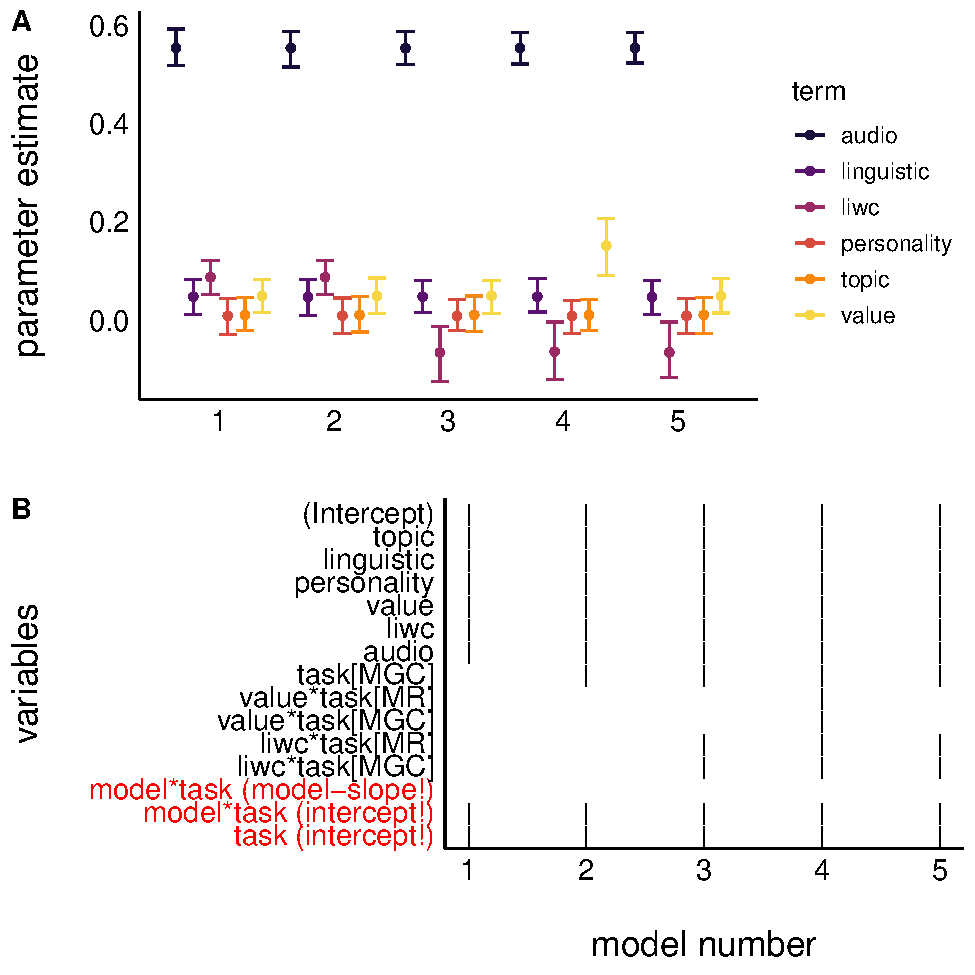
\includegraphics[width=\linewidth]{latex/figs/figure2.pdf}
    \caption{A: Parameter estimates of 5 hierarchical regression models. Error bars are 95\% confidence intervals, bootstrapped 500 times. B: Specific parameters that are estimated in the each of the models. Parameters that form the structure of the model are denoted both in red and with a ``!'' symbol, feature sets of primary interest are denoted in black, and variables for which two terms separated by a ``*'' are interaction terms.}
    \label{fig:parameterestimates}
\end{figure}

\section{Results}\label{sec:result}
% discussion regarding the results

\begin{figure}
    \centering
    % \includegraphics[width=\linewidth]{2020/latex/figs/interactions.pdf}
    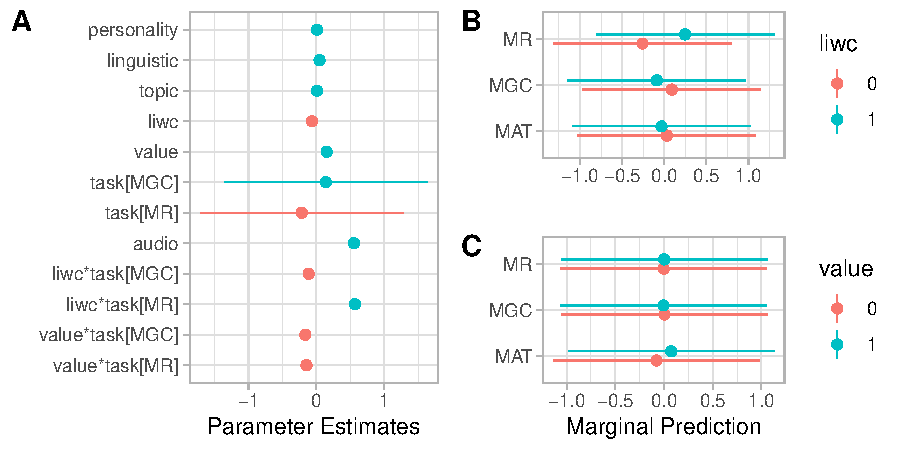
\includegraphics[trim={0mm 0 0 0},clip, width=\linewidth]{latex/figs/figure3.pdf}
    \caption{A: Parameter estimates of model 4. Error bars are 95\% confidence intervals. Interaction terms are denoted with the ``*'' symbol. B: Predicted scores for the inclusion of \emph{LIWC} on each of three MIR tasks, where 1 indicates that it was included and 0 indicates that it was not. C: Predicted scores for the inclusion of \emph{values} on each of three MIR tasks, where 1 indicates that it was included and 0 indicates that it was not.}
    \label{fig:parameterestimates4}
\end{figure}

We assessed models with two nested structures specified, where the parameters estimated are referred to as ``random effects''. The first included intercepts for each task, and the system used within task. The second estimated the same intercepts, and additionally estimated a slope for each system. For each of these two random effects structures, we then determined which parameters to estimate, referred to as ``fixed effects''. Specifically, we estimated parameters for each feature set, and interactions between all feature sets and the tasks. We first specified a ``maximal'' model, with all features and the task variable, and all two-way interactions among these variables. To remove unnecessary parameters, we ran a protocol which iteratively removed parameter estimates, retaining only those that either 1) significantly decrease model fit if not included, or 2) do not significantly decrease model fit if excluded. The Step function in the \emph{lmerTest} package, was used for this phase \cite{kuznetsova2017lmertest}. What remained were two interaction terms: the interaction between \emph{values} and task, and between \emph{LIWC} and task. As such, we estimated models with no interaction terms, as well as models with and without each of those interaction terms. When we assessed the interaction term, we also included the main effect of task. Thus, we also ran models with and without task included. The 5 models included for interpretation were those that converged without error. Parameter estimates are shown in Figure~\ref{fig:parameterestimates}A, and Figure~\ref{fig:parameterestimates}B shows which parameters were estimated in each model. For the full specification of our models, we refer readers to the reproducibility package\footnote{\url{https://github.com/mmc-tudelft/lyricpsych-ISMIR20}} accompanying this paper.

As is shown in Figure~\ref{fig:parameterestimates}A, we observe a consistent, large, positive effect of \emph{audio features} on the score, and no meaningful effects of \emph{topic} and \emph{personality} feature sets. Further, we observe a consistent, small, positive effect of \emph{values} across our specifications. This effect size increases in model 4, where the interaction between values and task was included. Similarly, \emph{LIWC} shows a small but positive effect, that appears to decrease when the interaction term of \emph{LIWC} and task is included. This suggests that \emph{LIWC} and \emph{values} may perform differently, depending on the task.

To clarify if this is the case, we examined the parameter estimates of model 4, which included interaction terms for both \emph{LIWC} and \emph{values} (see Figure~\ref{fig:parameterestimates4}A). Although both interaction terms were statistically significant, we observe that the confidence intervals for the main effect of task are very wide. This was expected, as 1) we were assessing an interaction effect which might increase the width of a the confidence interval, and 2) we were largely accounting for this variance by standardizing the score within each task, and by including task in the random effect structure. Figures~\ref{fig:parameterestimates4}A and~\ref{fig:parameterestimates4}B show the predicted values for both \emph{LIWC} and \emph{values} across tasks. Although the score was higher when \emph{LIWC} was included in the MR task and when \emph{values} was included in the MAT task, the predicted estimates are imprecise, as evidenced by the wide confidence intervals. As such, a more sensitive study design is likely required to obtain estimates of these interaction effects, e.g. analyses on individual dimensions of feature sets, to establish the most informative features, and/or more systems and more MIR tasks. Thus, we conclude that \emph{linguistic} and \emph{values} feature sets show the most consistent positive effects, and that \emph{LIWC} and \emph{values} may vary in performance based on task. 


\section{Limitations and Future Works}\label{sec:lim_fut}

Several limitations are still present in our current study. Firstly, although our feature sets did show promising yet small effect sizes, we did not assess the performance of individual dimensions. %This may account for variance in performance, as was observed with LIWC. 
Given that the feature sets vary greatly in both in terms of the number and content of sub-dimensions (see Table~\ref{tab:feat_dim}), reducing the overall set may result in a more sensitive set of features to examine.

Secondly, we did not consider subgroups of users, or of groups of songs. It may be possible that some users are more sensitive to the content of lyrics than others, and that lyric-sensitive users would benefit far more from lyric features than others. Further, it may be the case that lyrics are very important in some groups of songs vs. others (e.g Hip-Hop music vs. electronic dance music). Further research could examine the potential existence of a lyric-sensitive sub-group of users, lyric-sensitive songs, and how these two may interact.

Thirdly, aspects of our experimental design can be elaborated in future work: 1) Although we strategically sampled a limited number of MIR tasks and a limited number of systems, we  did not fully address all possibilities. For instance, future work can include more contemporary systems such as deep learning, thereby increasing generalizability of our results. 2) Certain task metrics could be improved, although we strategically designed our experiment to prevent local noise from skewing our conclusions: e.g.\ a different performance measure for the genre classification (i.e. AUC-ROC) could deliver a more accurate experimental result, given its skewed class distribution.

Lastly, the reliability of all of our feature sets could be better assessed in the future. This is particularly true of our \emph{personality} features: they contain words that have been shown to describe individuals that have or lack in personality traits, but it is not clear that individuals with those traits use the specific words that describe them. 

\section{Conclusion}\label{sec:conclusion}
% and conclusion

Although the \emph{audio} features in our analysis most positively affected performance on various MIR tasks, our lyric-based text features did show some promise. More specifically, \emph{linguistic} and \emph{values} feature sets showed consistent, small effect sizes. Given that the interactions between \emph{LIWC} and task were significant, it may be the case that \emph{LIWC} features are also useful. We can conclude that text-based features drawn from Psychology literature anticipate further research, and that further investigations addressing the current limitations will lead to better data-driven understanding of the role lyrics play in music consumption.
% \footnote{A reproducibility package for this paper, including complete code base, analytical scripts, data, and notes, can be found at \url{https://github.com/mmc-tudelft/lyricpsych-ISMIR20}.} 


\section{Acknowledgement}\label{sec:ack}
This work was carried out on the Dutch national e-infrastructure with the support of SURF Cooperative. 


% For bibtex users:
\bibliography{ISMIRtemplate}

% For non bibtex users:
%\begin{thebibliography}{citations}
%
%\bibitem {Author:00}
%E. Author.
%``The Title of the Conference Paper,''
%{\it Proceedings of the International Symposium
%on Music Information Retrieval}, pp.~000--111, 2000.
%
%\bibitem{Someone:10}
%A. Someone, B. Someone, and C. Someone.
%``The Title of the Journal Paper,''
%{\it Journal of New Music Research},
%Vol.~A, No.~B, pp.~111--222, 2010.
%
%\bibitem{Someone:04} X. Someone and Y. Someone. {\it Title of the Book},
%    Editorial Acme, Porto, 2012.
%
%\end{thebibliography}

\end{document}

